\documentclass{article}

\usepackage[top=2in, bottom=1.5in, left=1in, right=1in]{geometry}
\usepackage{fancyhdr} 		% page header
\usepackage{amsmath}
\usepackage{amssymb}
\usepackage{float}
\usepackage{graphicx}
\usepackage{url}
\usepackage{tikz}
\usetikzlibrary{shapes.geometric}
\usetikzlibrary{positioning}
\usepackage{hyperref}

\pagestyle{fancy} 
\fancyhf{}
\fancyhead[L]{CS 540}
\fancyhead[R]{Fall 2017}

\def\x{\mathbf{x}}
\def\y{\mathbf{y}}
\def\w{\mathbf{w}}
\def\p{\mathbf{p}}

\begin{document}

\begin{center}
{\bf \large CS 540: HW5

Jurijs Nazarovs}
\end{center}

\vspace{1cm}



\section*{Question 1: Game Tree Search [60 points]}



\begin{enumerate}

\item  Minimax algorithm on this game tree

   \begin{figure}[ht]
\centering
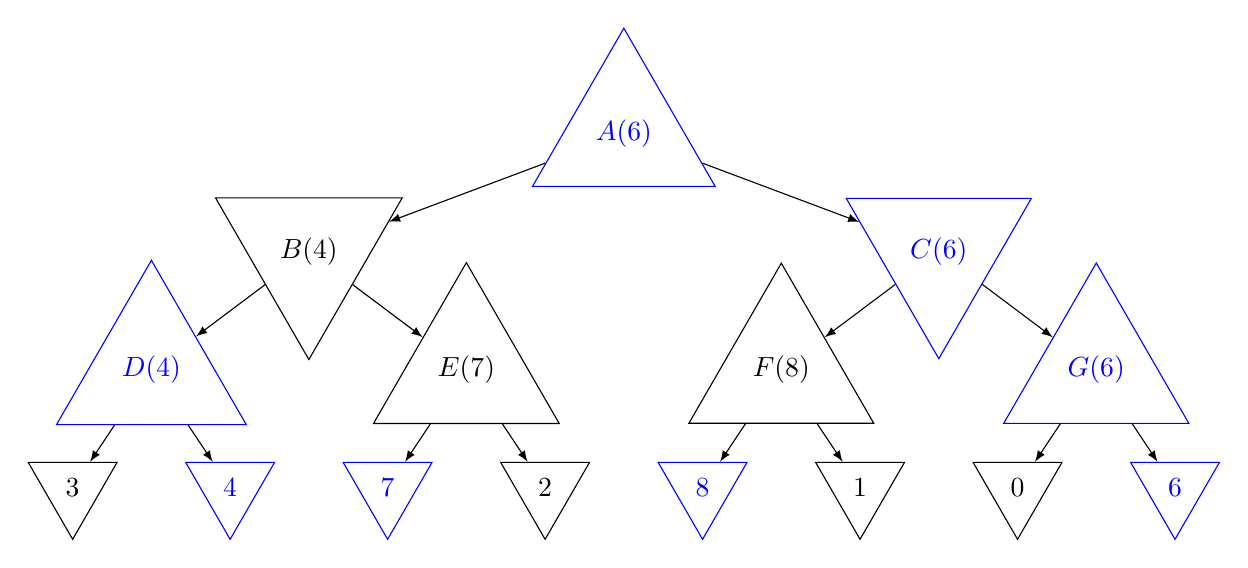
\begin{tikzpicture}[edge from parent/.style={draw,-latex},
    triangle/.style = {regular polygon, regular polygon sides=3},
    border rotated/.style = {shape border rotate=180},
    level distance=1.5cm,
    level 1/.style={sibling distance=8cm},
    level 2/.style={sibling distance=4cm},
    level 3/.style={sibling distance=2cm}]
    \node [triangle,draw, blue]{$A(6)$}
        child {node [triangle,border rotated,draw]{$B(4)$}
            child {node [triangle,draw, blue]{$D(4)$}
                child {node [triangle,border rotated,draw]{$3$}}
                child {node [triangle,border rotated,draw, blue]{$4$}}
            }
            child {node [triangle,draw]{$E(7)$}
                child {node [triangle,border rotated,draw, blue]{$7$}}
                child {node [triangle,border rotated,draw]{$2$}}
                }
        }
        child {node [triangle,border rotated,draw, blue]{$C(6)$}
            child {node [triangle,draw]{$F(8)$}
                child {node [triangle,border rotated,draw, blue]{$8$}}
                child {node [triangle,border rotated,draw]{$1$}}
                }
            child {node [triangle,draw, blue]{$G(6)$}
                child {node [triangle,border rotated,draw]{$0$}}
                child {node [triangle,border rotated,draw, blue]{$6$}}
                }
        };
\end{tikzpicture}
\end{figure}


\newpage
\item Alpha-beta pruning to compute the Minimax value at each node for the original game tree

Order of numbers in node is (theoretical value, $\alpha$, $\beta$). 

\begin{figure}[H]
\centering
\resizebox{.7\totalheight}{!}{%
\begin{tikzpicture}[edge from parent/.style={draw,-latex},
    triangle/.style = {regular polygon, regular polygon sides=3},
    border rotated/.style = {shape border rotate=180},
    level distance=4cm,
    level 1/.style={sibling distance=10cm},
    level 2/.style={sibling distance=4.5cm},
    level 3/.style={sibling distance=2.5cm}]
    \node [triangle,draw]{$A(6, 6, \infty)$}
        child {node [triangle,border rotated,draw]{$B(4,-\infty, 4)$}
            child {node [triangle,draw]{$D(4,4,\infty)$}
                child {node [triangle,border rotated,draw]{$3$}}
                child {node [triangle,border rotated,draw]{$4$}}
            }
            child {node [triangle,draw]{$E(7,7,4)$}
                child {node [triangle,border rotated,draw]{$7$}}
                child {node [triangle,border rotated,draw, red]{$2$}edge from parent node[right, draw=none, red]{\huge{\textbf{X}}}}
                }
        }
        child {node [triangle,border rotated,draw]{$C(6,4,6)$}
            child {node [triangle,draw]{$F(8,8,\infty)$}
                child {node [triangle,border rotated,draw]{$8$}}
                child {node [triangle,border rotated,draw]{$1$}}
                }
            child {node [triangle,draw]{$G(6,6,8)$}
                child {node [triangle,border rotated,draw]{$0$}}
                child {node [triangle,border rotated,draw]{$6$}}
                }
        };
\end{tikzpicture}
}
\end{figure}

\item Pruned branches
Pruned branches/nodes are highlighted with red color on a graph above. Namely, it is a node with value 2, child of node E.

\item Why we would want to use alpha-beta pruning?

We would want to use alpha-beta pruning to avoid going threw branches, which cannot make situation better. Such approach saves time in a tree
analysis.

\item  Probability of a player choosing an optimal action at each node?
At every node the probability  to choose an optimal action is  $P = 0.5+0.5^2= 0.75$.


\newpage
\item Chance node

   \begin{figure}[H]
\centering
\resizebox{1.3\totalheight}{!}{%
\begin{tikzpicture}[edge from parent/.style={draw,-latex},
    triangle/.style = {regular polygon, regular polygon sides=3},
    border rotated/.style = {shape border rotate=180},
    level distance=2cm,
    level 2/.style={sibling distance=10cm},
    level 4/.style={sibling distance=6cm},
    level 6/.style={sibling distance=2cm}]
    \node [triangle,draw]{$A$}
    child{node [circle,draw]{$A'$}
        child {node [triangle,border rotated,draw]{$B$}
        child {node [circle,draw]{$B'$}
            child {node [triangle,draw, blue]{$D$}
            child {node [circle,draw]{$D'$}
                child {node [triangle,border rotated,draw]{$3$} edge from parent node[left, draw=none]{$0.25$}}
                child {node [triangle,border rotated,draw, blue]{$4$} edge from parent node[right, draw=none]{$0.75$}}
            }
             edge from parent node[left, draw=none]{$0.75$}
            }
            child {node [triangle,draw]{$E$}
            child {node [circle,draw]{$E'$}
                child {node [triangle,border rotated,draw, blue]{$7$} edge from parent node[left, draw=none]{$0.75$}}
                child {node [triangle,border rotated,draw]{$2$} edge from parent node[right, draw=none]{$0.25$}}
            }
            edge from parent node[right, draw=none]{$0.25$}
            }
        }      
        edge from parent node[left, draw=none]{$0.25$}  
        }
        child {node [triangle,border rotated,draw, blue]{$C$}
        child {node [circle,draw]{$C'$}
            child {node [triangle,draw]{$F$}
            child {node [circle,draw]{$F'$}
                child {node [triangle,border rotated,draw, blue]{$8$} edge from parent node[left, draw=none]{$0.75$}}
                child {node [triangle,border rotated,draw]{$1$} edge from parent node[right, draw=none]{$0.25$}}
                }
                edge from parent node[left, draw=none]{$0.25$}
                }
            child {node [triangle,draw, blue]{$G$}
            child {node [circle,draw]{$G'$}
                child {node [triangle,border rotated,draw]{$0$} edge from parent node[left, draw=none]{$0.25$}}
                child {node [triangle,border rotated,draw, blue]{$6$} edge from parent node[right, draw=none]{$0.75$}}
                }
                edge from parent node[right, draw=none]{$0.75$}
                }
        }
        edge from parent node[right, draw=none]{$0.75$}
        }
        };
\end{tikzpicture}
}
\end{figure}

    
\newpage
\item Non-deterministic game. Expected value is provided in the brackets for every node.
\begin{figure}[H]
\centering
\resizebox{0.65\totalheight}{!}{%
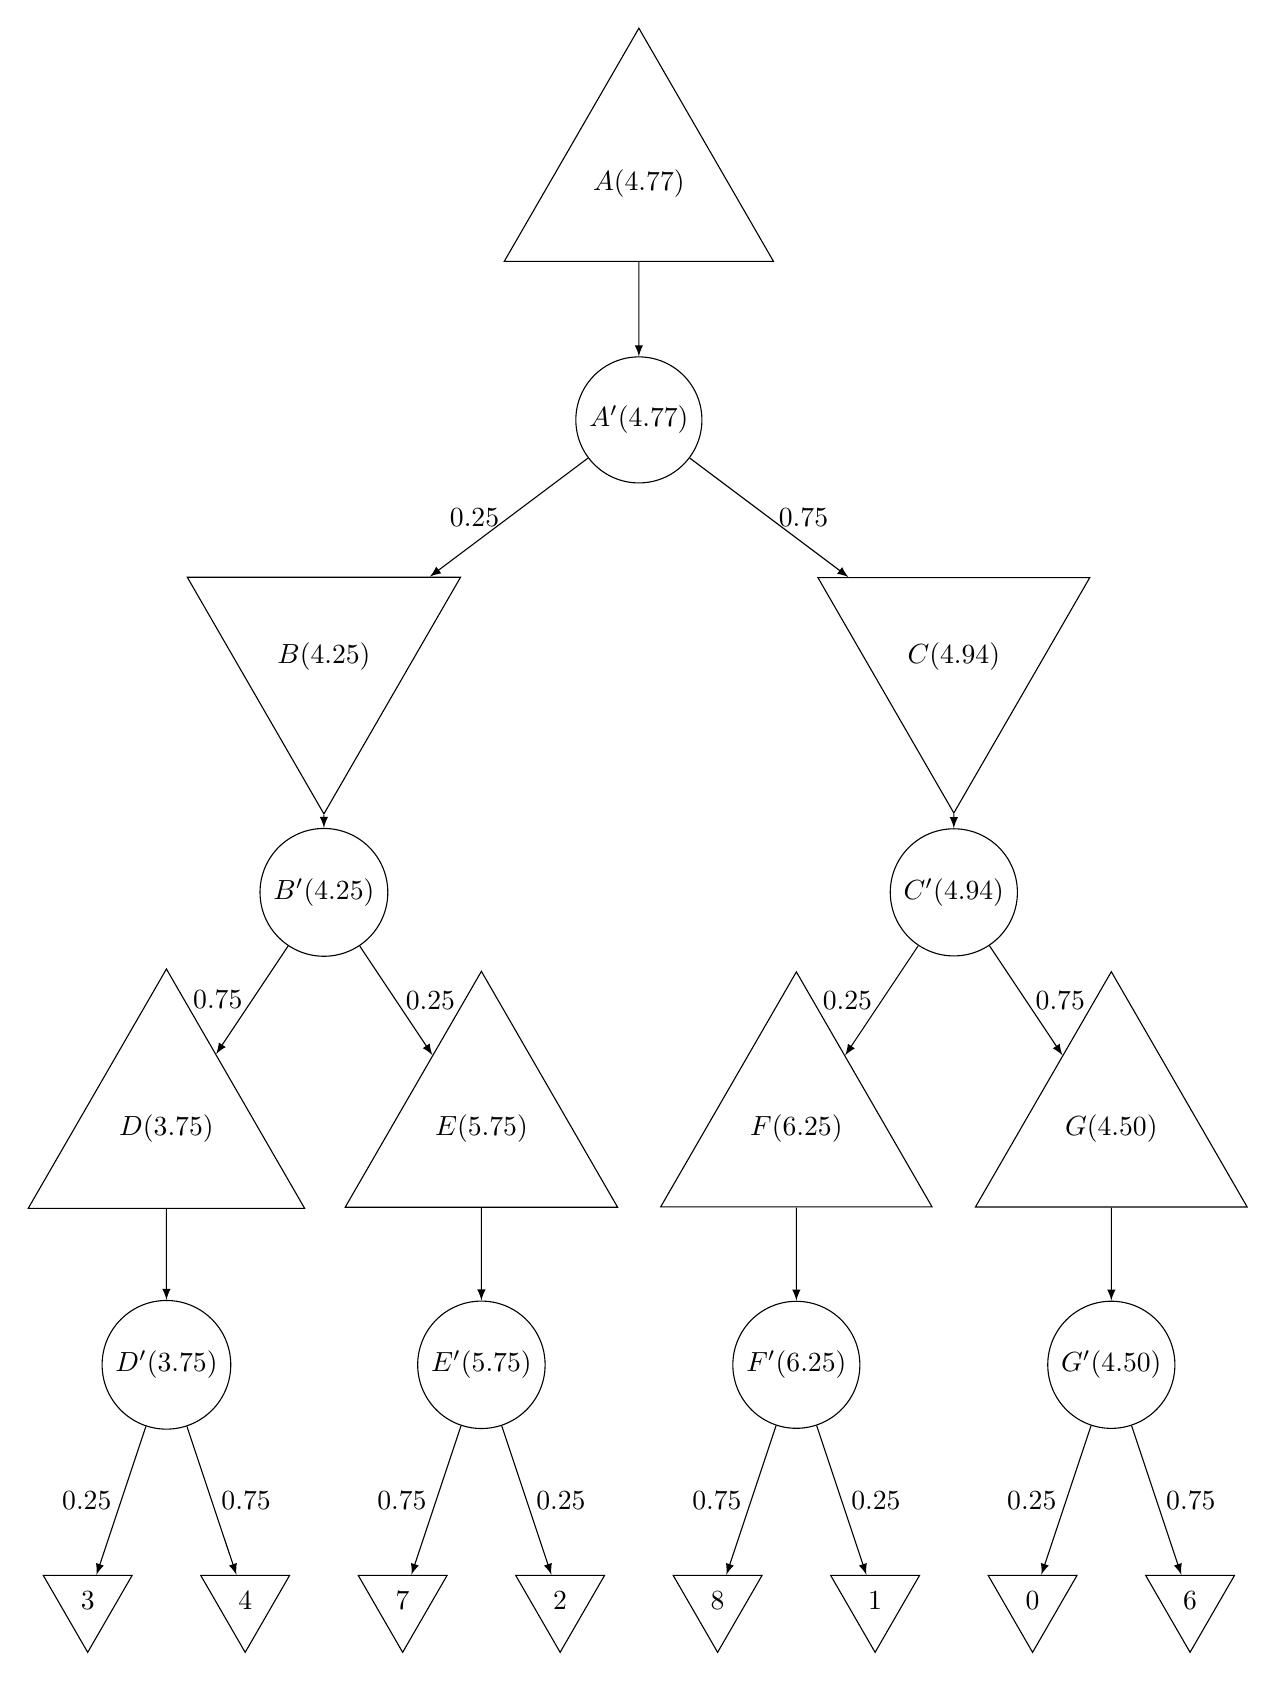
\begin{tikzpicture}[edge from parent/.style={draw,-latex},
    triangle/.style = {regular polygon, regular polygon sides=3},
    border rotated/.style = {shape border rotate=180},
    level distance=3cm,
    level 2/.style={sibling distance=8cm},
    level 4/.style={sibling distance=4cm},
    level 6/.style={sibling distance=2cm}]
    \node [triangle,draw]{$A(4.77)$}
    child{node [circle,draw]{$A'(4.77)$}
        child {node [triangle,border rotated,draw]{$B(4.25)$}
        child {node [circle,draw]{$B'(4.25)$}
            child {node [triangle,draw]{$D(3.75)$}
            child {node [circle,draw]{$D'(3.75)$}
                child {node [triangle,border rotated,draw]{$3$} edge from parent node[left, draw=none]{$0.25$}}
                child {node [triangle,border rotated,draw]{$4$} edge from parent node[right, draw=none]{$0.75$}}
            }
             edge from parent node[left, draw=none]{$0.75$}
            }
            child {node [triangle,draw]{$E(5.75)$}
            child {node [circle,draw]{$E'(5.75)$}
                child {node [triangle,border rotated,draw]{$7$} edge from parent node[left, draw=none]{$0.75$}}
                child {node [triangle,border rotated,draw]{$2$} edge from parent node[right, draw=none]{$0.25$}}
            }
            edge from parent node[right, draw=none]{$0.25$}
            }
        }      
        edge from parent node[left, draw=none]{$0.25$}  
        }
        child {node [triangle,border rotated,draw]{$C(4.94)$}
        child {node [circle,draw]{$C'(4.94)$}
            child {node [triangle,draw]{$F(6.25)$}
            child {node [circle,draw]{$F'(6.25)$}
                child {node [triangle,border rotated,draw]{$8$} edge from parent node[left, draw=none]{$0.75$}}
                child {node [triangle,border rotated,draw]{$1$} edge from parent node[right, draw=none]{$0.25$}}
                }
                edge from parent node[left, draw=none]{$0.25$}
                }
            child {node [triangle,draw]{$G(4.50)$}
            child {node [circle,draw]{$G'(4.50)$}
                child {node [triangle,border rotated,draw]{$0$} edge from parent node[left, draw=none]{$0.25$}}
                child {node [triangle,border rotated,draw]{$6$} edge from parent node[right, draw=none]{$0.75$}}
                }
                edge from parent node[right, draw=none]{$0.75$}
                }
        }
        edge from parent node[right, draw=none]{$0.75$}
        }
        };
\end{tikzpicture}
}
\end{figure}


\end{enumerate}


\section*{Question 2: Natural Language Processing [40 points, 5 points each]}
\begin{enumerate}

\item I believe that the most convenient way to break the corpus into ``computer words" is to use bash or analogue languages, since there is a lot 
of tools to work with text-processing. We can simply concatenate all files inside a directory, translate spaces into ``new line" character, and 
proceed with sorting and unique commands using pipeline. Thus, as a word we consider a sequence of characters between spaces.

One - line command, which takes just 0.38s, is: 
\begin{verbatim}
cat "$dir"/* | tr [:space:] "\n" | grep '[^[:blank:]]' | sort | uniq -c | sort -bgr > sorted.list
\end{verbatim}

Such program allows to add additional editing features, by applying more commands in pipeline. For example, we can make all words
not case sensitive, or delete commas and other signs by adding command tr, e.g. tr ``[:lower:]" ``[:upper:]".

\item 
Total words:  205057\\
Unique words: 18383

\item  Top 20 word types and their counts.

10636 the\\
6686 to\\
6128 of\\
5157 and\\
3846 in\\
3702 a\\
3354 that\\
3312 is\\
2663 be\\
2567 AI\\
2022 will\\
1615 for\\
1613 are\\
1517 it\\
1505 not\\
1483 on\\
1483 as\\
1221 with\\
1140 The\\
1066 have\\

\item Pick 20 bottom word types and their counts.

   1 "NLP\\
   1 "NHE-Fact-Sheet."\\
   1 "M�canique\\
   1 "Meditations\\
   1 "Mars".\\
   1 "Large-scale\\
   1 "Given\\
   1 "Ethical\\
   1 "Current\\
   1 "Competition\\
   1 "Changes\\
   1 "Bad\\
   1 "Back\\
   1 "Autonomous\\
   1 "As\\
   1 "ARTIFICIAL\\
   1 "A\\
   1 "2016\\
   1 "..on\\
   1 "...\\



\item  Plot $r$ on the x-axis and $c$ on the y-axis, namely each $(r_i, c_i)$ is a point in that 2D space (you can choose to connect the points or not).

\begin{figure}[H]
\centering
\includegraphics[width=\textwidth]{rawData.pdf}
\caption{No scaling}
\end{figure}

\item Plot $\log(r)$ on the x-axis and $\log(c)$ on the y-axis. 

\begin{figure}[H]
\centering
\includegraphics[width=\textwidth]{logData.pdf}
\caption{Log scaling for both variables}
\end{figure}

\item Briefly explain what the shape of the two curves mean.

Both curves are non-increasing curves. Which shows that higher rank corresponds to lower count. From the plot of raw data, we can see that
counts and rank are described by following relation: $\text{count} = \frac{1}{\text{rank}} $. Such observation is consistent with Zipf's Law, described in lectures as $f \propto \frac{1}{g}$. 

Since from first picture we can assume that $\text{count} = \frac{1}{\text{rank}} $ , then $\text{log(count)} = -\text{log(rank)} $. That is why we see the negative slope of the graph on second image.   And the graph looks more as a linear function rather the hyperbola. 

\item Discuss \emph{two} potential major issues with your computer words, if one wants to use them for natural language processing.

1. Difference in  character encoding standards of separate documents. I noticed that sometimes ' is presented as is, but sometime it is shown as 
$<92>$. Such issue leads to wrong results of counting values.

2. Since I considered just a sequence of characters between spaces as a word, and not any of regular expressions, my program does not count for misspellings. Which might cause outliers in counts. Also, for the same reason, words combined with some symbols like " or commas are considered as different from just words.

\end{enumerate}

\end{document}
